\chapter{Simulation study}
\label{chap:SimulationStudy}

\section{Introduction}
In order to study the methods in more depth a simulation study was performed. The main advantage of this simulation study over using real species, as was done in Chapter \ref{ch:Applications}, is that we can decide on which variables make up the model. Because of the usual non-linear shape of the response-functions, the sampling design, \dots it is quite hard to set up a simulation study. Luckily the
\textsc{virtualspecies} package \parencite{virtualspecies, leroy_virtualspecies_2015} provides a simulation framework that includes important characteristics of species' distributions.\\

\section{Overview of the \textsc{virtualspecies} package and the simulation set-up}

First of all, the \textsc{virtualspecies} package generates a suitability raster, i.e.\ a raster containing high values for suitable habitat and vice versa, based upon a set of provided rasters. Since the package imposes no restrictions on the function that generates the suitability the suitability raster has to be converted into a probability of occurrence map. This can be done by using e.g.\ the logit function to map $\mathbb{R} \to [0,1]$. Once a probability map is obtained a raster containing $1$ where the simulated species is present and $0$ otherwise can be obtained by sampling cells with a probability proportional to the probability of the occurrence map. Finally from this raster we can obtain a presence-only sample by using a drawing random points within the cells that have a value of $1$ in the species distribution raster.\\


To facilitate the computations it was decided to select one area in which several random species were generated. In order to make sure that the environmental conditions can fluctuate within the distribution of one generated species to the next it was required that the selected area has to contain different types of habitat types. The obvious choice would be to use the contiguous 47, however this has a huge computational demands. In the end it was decided to to perform the simulation study on data contained within a rectangle that approximately corresponds to Washington state, see Figure \ref{fig:WashState}. Washington state has a big precipitation and temperature gradient because of the rain shadow created by the Cascade Range. This is also reflected in the fact that the types of habitat within this extent range from temperate rainforests, e.g.\ the Hoh Rainforest, to steppe- and dessert-like areas in Southeastern Washington. \\

\begin{figure}[!htb]
\center
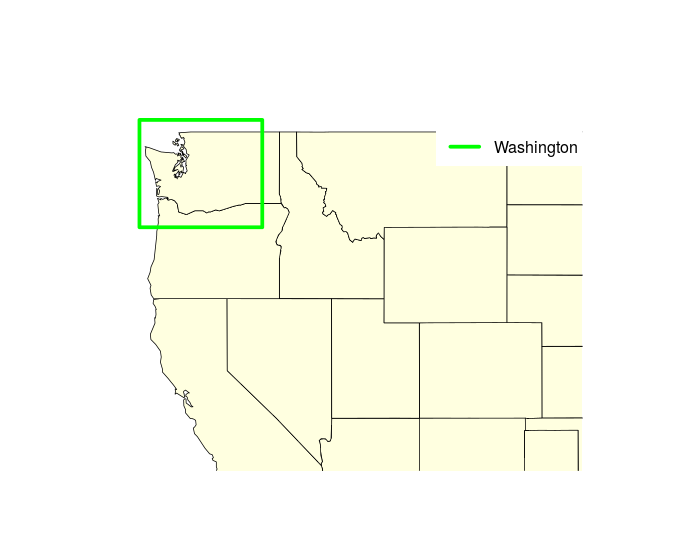
\includegraphics[scale=0.5]{Plots/WashingtonPlot.png}
\caption{\label{fig:WashState}Extent considered in the simulation study.}
\end{figure}

In order to study the generalizability of the methods it was decided that $5$ different species would be simulated. Furthermore, to be able to investigate the sample to sample variability of each method $5$ different presence-only samples were drawn for each simulated species. Since the mean (resp.\ median) number of observations of the presence-only datasets is $320.3$ (resp.\ $133.5$) it was decided to simulate $200$ occurrence points for each simulated dataset. \\

In Section \ref{sec:AUC} the various sources of the variability in the AUC values were discussed. Given that the interest is mainly in the training sample to training sample variability it was decided to try to restrict the test sample to test sample variability to some extent. This can be done by taking a large test set. Using a sample of $1000$ occurrence and $1000$ background locations the standard error of the AUC value, conditional on the classifier, is $\approx 0.013$. This should 

\section{Results}

\section{Discussion}





